\documentclass{beamer}

\usepackage{xspace}

 \usepackage{calc}                                             %%
    \usepackage{multirow}                                         %%
    \usepackage{hhline}                                           %%
    \usepackage{ifthen}   
\usepackage{listings}
\usepackage[latin1]{inputenc}
    \usepackage{color}                                            %%
    \usepackage{array}                                            %%
    \usepackage{longtable}                                        %%
  
\newcounter{saveenumi}
\newcommand{\seti}{\setcounter{saveenumi}{\value{enumi}}}
\newcommand{\conti}{\setcounter{enumi}{\value{saveenumi}}}                                      

\setbeamertemplate{caption}[numbered]{}
    
\providecommand{\pr}[1]{\ensuremath{\Pr\left\{#1\right\}}}
\providecommand{\brak}[1]{\ensuremath{\left(#1\right)}}
\providecommand{\cbrak}[1]{\ensuremath{\left\{#1\right\}}}
\providecommand{\sbrak}[1]{\ensuremath{{}\left[#1\right]}}                                             %


% Theme choice:
\usetheme{Madrid}

% Title page details: 
\title{\textbf{Mess Food Usage by IITH Student Community} \\
MA4240:Applies Statistics - Group Project}
\author{Blessy Anvitha \quad Saanvi Amrutha \quad Anirudh Srinivasan \quad Arnav Asati\\ Lokesh Surana \quad Bhanu Prasad \quad Samar Singhai \quad Shivanand}
\date{\today}
\logo{\large \LaTeX{}}


\begin{document}

% Title page frame
\begin{frame}
    \titlepage 
\end{frame}

% Remove logo from the next slides
\logo{}
\author{}

% Outline frame
\begin{frame}{Outline}
    \tableofcontents
\end{frame}

% Outline frame
\section{Introduction}
\begin{frame}{Introduction}
\begin{block}{}
Through this project we tried to understand \textbf{how the students of IIT Hyderabad are using the mess food}. We tried observing if the student community is properly using the mess food or there's a lot wastage. Most of the possible variables that effect the usage like reasons for skipping mess, degree the student pursuing, financial status, etc., are being asked for in the survey conducted. For drawing the results we opted observational study, We tried including all the possible groups and hence assuming that the data is a random population sample.
\end{block}
\end{frame}

\section{Variables of Interest}
\begin{frame}{Variables of Interest}
\begin{block}{}
\begin{enumerate}
\item{How many times a week you skip eating mess food?}
\item{Early sleeping or Late-night sleeping?}
\item{Which meal do you usually skip in a day?}
\item{Are you a vegetarian or non-vegetarian?}
\item{Food Preference?}
\item{What are the reasons for you to skip?}
\item{What are you pursuing?}
\item{What department are you in?}
\item{Gender and Age?}
\item{Family Financial Status?}
\item{What's your preferable alternative?}
\end{enumerate}
\end{block}
\end{frame}

\section{Data Visualization}
\begin{frame}{Data Visualization}
\begin{block}{Analyzing the Uni-variate Numerical dataset}
    \begin{table}[!h]
    \centering
\caption{How many times a week you skip eating mess food? }
\label{tab:table_label}
    \begin{tabular}{|c|c|c|} 
                 \hline 
        $count$               &$300$     
        
        \\ \hline
        $Mean$   &$7.296$      \\ \hline    
        $Median$    &$6.5$      \\ \hline
        $Mode$       &$10$       \\\hline
        $Std$       &$4.73$ \\\hline
        $Min$       &  $0$ \\\hline
        $25\%$       &$3.5$ \\\hline
        $50\%$       & $6.5$ \\\hline
        $75\%$       &$10$ \\\hline
        $Max$       &$21$ \\ \hline
    \end{tabular}
\end{table}
\end{block}
\end{frame}
\begin{frame}{Data Visualization}
\begin{block}{Box Plot}
\begin{figure}[H]
    \centering
    \caption{plot of uni-variate numerical dataset}
    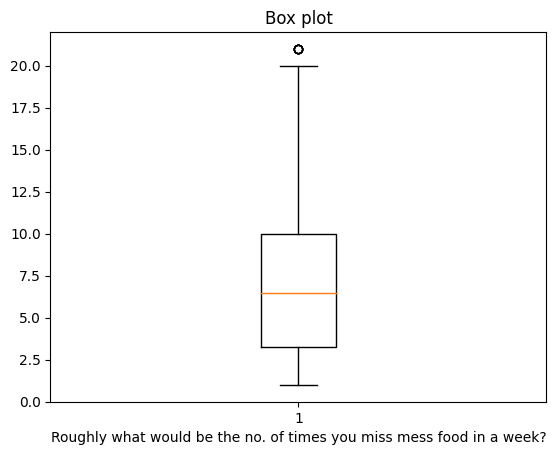
\includegraphics[scale = 0.55]{boxplot.png} 
    \label{fig:boxplot}
\end{figure}
\end{block}
\end{frame}

\begin{frame}{Data Visualization}
\begin{block}{Male vs Female}
\begin{figure}
      \centering
    \caption{Side-by-Side Boxplot}
    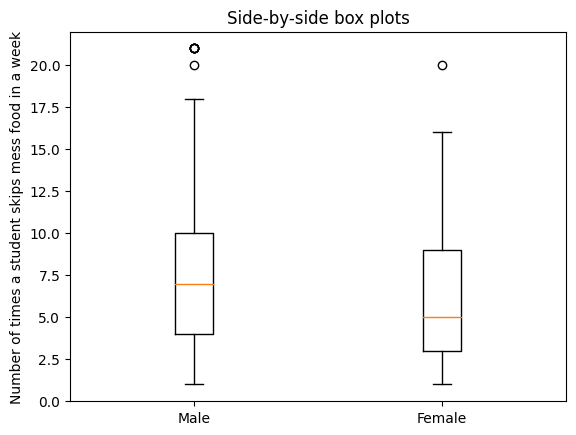
\includegraphics[scale = 0.55]{side-by-side.png}  
    \label{fig:side-by-side}
\end{figure}
\end{block}
\end{frame}
\begin{frame}{Data Visualization}
\begin{block}{Normality plot}
\begin{figure}[H]
     \centering
     \caption{Analysing whether the univariate numerical dataset is normally distributed or not }
    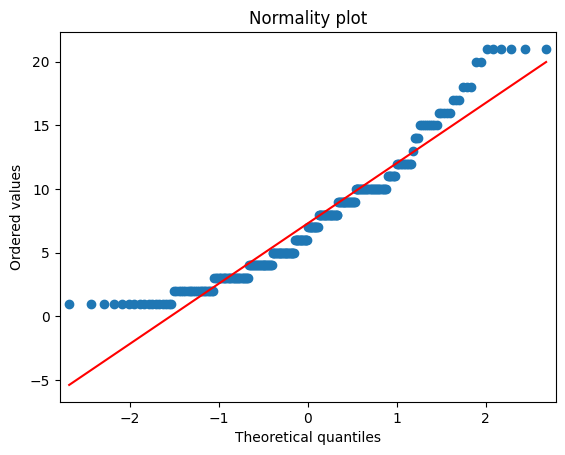
\includegraphics[scale = 0.54]{normality_plot.png} 
    \label{Normality_plot}
\end{figure}
\end{block}
\end{frame}
\begin{frame}{Exploratory Data Analysis}
\begin{block}{Frequency of skipping mess}
\begin{figure}
      \centering
    \caption{Frequency of Number of times Meal skip }
    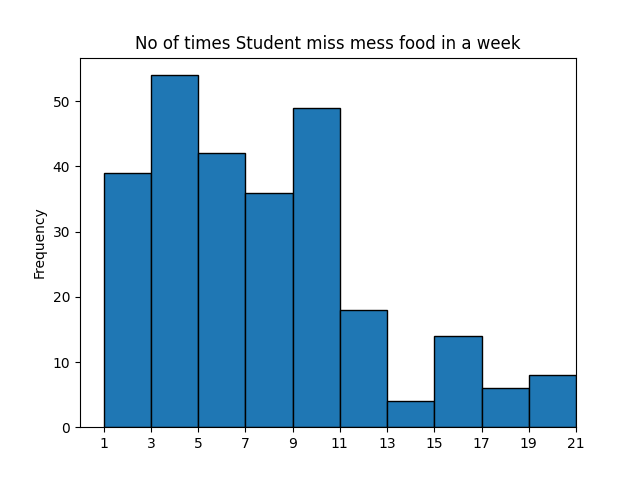
\includegraphics[scale = 0.55]{histogram_meal_skip.png}  
    \label{histogram_meal_skip}
\end{figure}
\end{block}
\end{frame}
% ########################
\begin{frame}{Exploratory Data Analysis}
\begin{block}{Participation based on degree}
\begin{figure}
      \centering
    \caption{Degree vs number of responses }
    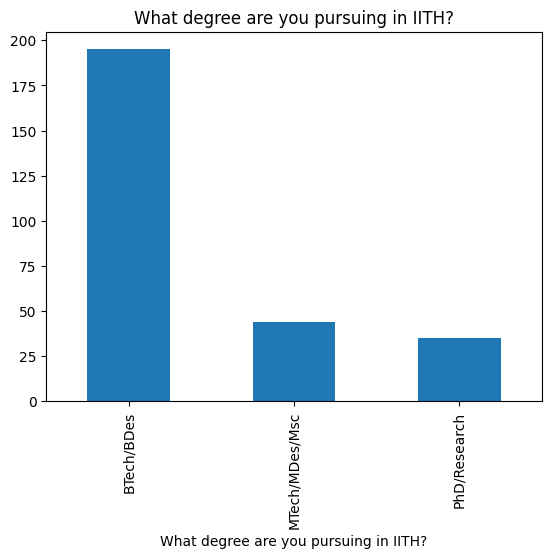
\includegraphics[scale = 0.55]{bar_degree.png}  
    \label{fig:side-by-side}
\end{figure}
\end{block}
\end{frame}
\begin{frame}{Exploratory Data Analysis}
\begin{block}{Participation based on branch}
\begin{figure}
      \centering
    \caption{Branch vs number of responses}
    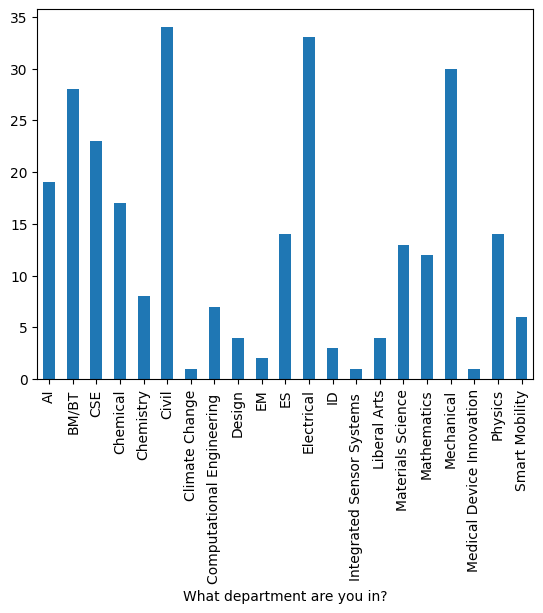
\includegraphics[scale = 0.55]{bar_department.png}  
    \label{fig:side-by-side}
\end{figure}
\end{block}
\end{frame}
\begin{frame}{Exploratory Data Analysis}
\begin{block}{Involvement in terms of gender}
\begin{figure}
      \centering
    \caption{Male responses vs female responses}
    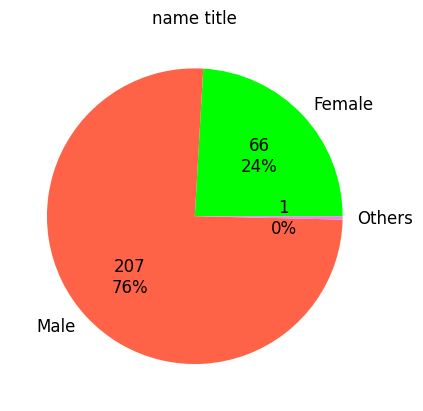
\includegraphics[scale = 0.55]{pie_gender.png}  
    \label{fig:side-by-side}
\end{figure}
\end{block}
\end{frame}
\begin{frame}{Exploratory Data Analysis}
\begin{block}{Economic classes}
\begin{figure}
      \centering
    \caption{Share of different economic classes}
    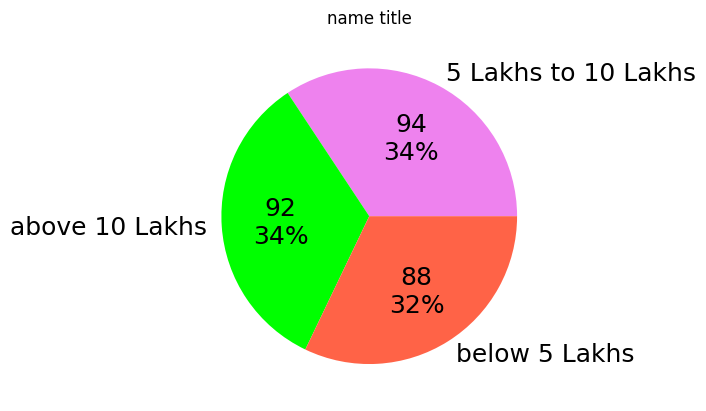
\includegraphics[scale = 0.55]{pie_income.png}  
    \label{fig:side-by-side}
\end{figure}
\end{block}
\end{frame}
\begin{frame}{Exploratory Data Analysis}
\begin{block}{Majority are late night sleepers!!}
\begin{figure}
      \centering
    \caption{Early sleepers vs Late sleepers}
    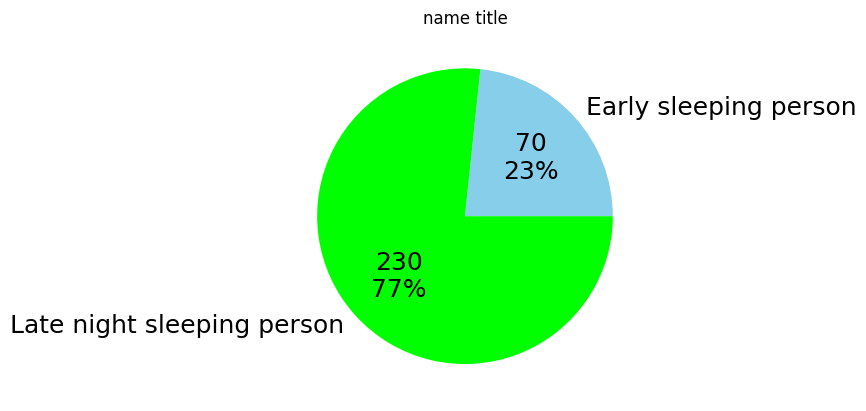
\includegraphics[scale = 0.55]{pie_sleep_categoty.png}  
    \label{fig:side-by-side}
\end{figure}
\end{block}
\end{frame}
\begin{frame}{Exploratory Data Analysis}
\begin{block}{Non-veg vs veg}
\begin{figure}
      \centering
    \caption{Share of non-veg and veg}
    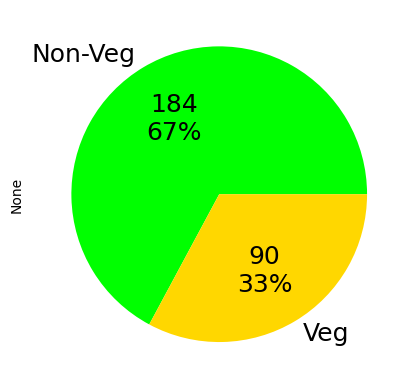
\includegraphics[scale = 0.55]{pie_veg_non-veg.png}  
    \label{pie_veg_non_veg}
\end{figure}
\end{block}
\end{frame}
% *******************************************8
\begin{frame}{Data Analysis}
\begin{block}{Which meal is being skipped the most??}
\begin{figure}
      \centering
    \caption{Meal skip vs type of meal }
    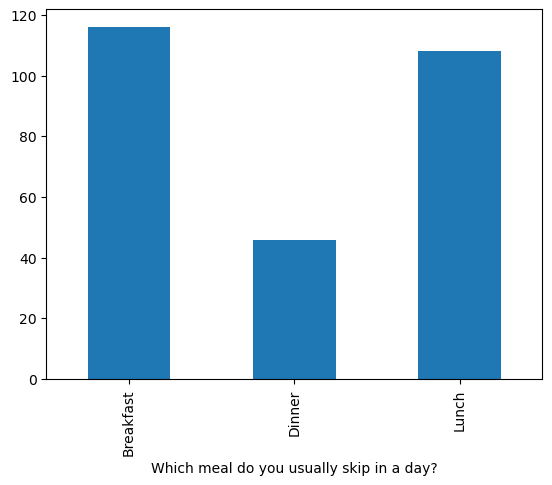
\includegraphics[scale = 0.55]{bar_timing_skip.png}  
    \label{bar_timing_skip}
\end{figure}
\end{block}
\end{frame}
\begin{frame}{Data Analysis}
\begin{block}{Which food is preferred the most?}
\begin{figure}
      \centering
    \caption{ Preference of Regional food}
    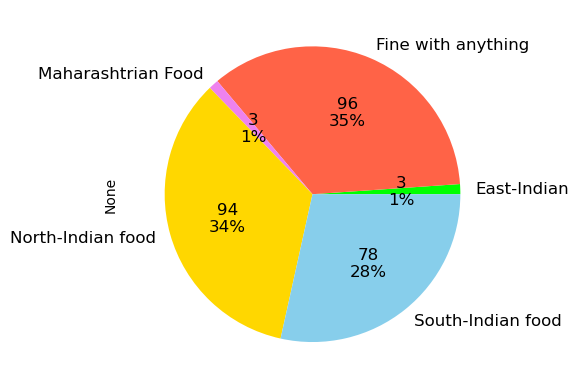
\includegraphics[scale = 0.55]{pie_food_pref.png}  
    \label{pie_food_pref}
\end{figure}
\end{block}
\end{frame}
\begin{frame}{Data Analysis}
\begin{block}{Impact of working days}
\begin{figure}
      \centering
    \caption{Meal skip based on part of the week }
    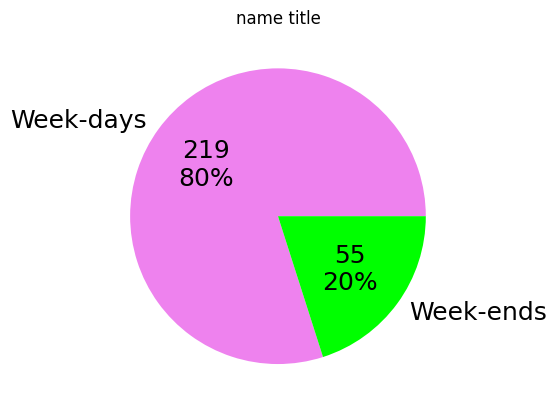
\includegraphics[scale = 0.55]{pie_plot_weekdays.png}  
    \label{pie_weekdays}
\end{figure}
\end{block}
\end{frame}
\begin{frame}{Data Analysis}
\begin{block}{Number of times mess is skipped}
\begin{figure}
      \centering
    \caption{Range frequency mess is skipped }
    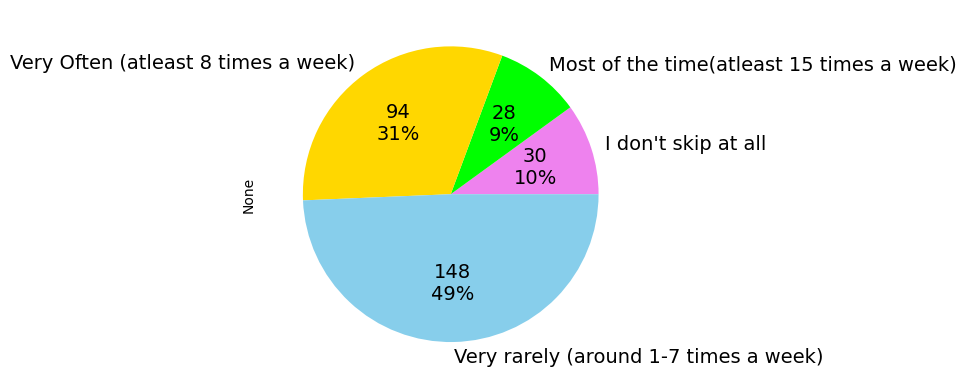
\includegraphics[scale = 0.55]{pie_skip_categoty.png}  
    \label{pie_skip}
\end{figure}
\end{block}
\end{frame}

\section{Class Interval Estimation}
\begin{frame}{Class Interval Estimation}
    \begin{block}{}
        \item \textbf{Case-1: Confidence Interval of $\mu$, where $\mu$ is the mean number of meals skipped by a student at IITH in a week. } \\
       Consider a random sample of size $n = 50$. 
       Sample mean and sample standard deviation are $\bar{x}$ and $S$ respectively, where
        \begin{align*}
            \bar{x}= 6.98, 
            S = 4.18 
        \end{align*}       
      
Also, for a $95\%$ CI, $\alpha=0.05$,$t_{\alpha/2,n-1} =t_{0.025,49}=2.0096$ \\
Now, the resulting $95\%$ CI is:
      \begin{align*}
        \bar{x}-t_{\alpha/2,n-1}\left(\frac{S}{\sqrt{n}}\right) &\leq \mu \leq \bar{x}+t_{\alpha/2,n-1}\left(\frac{S}{\sqrt{n}}\right)\\
        5.792 &\leq \mu \leq 8.168
      \end{align*}
      Thus, based on the sample data, CI of mean number of meals skipped by a student in a week is $[5.792,8.168]$ 
      \end{block}
\end{frame}
\begin{frame}{Class Interval Estimation}
    \begin{block}{}
        \item \textbf{Case-2: CI of $\sigma$,where $\sigma$ is the standard deviation of the population.} \\
       Consider a random sample of size $n = 50$.   \\
       Here sample variance,    $S^2 = 17.49$  \\
       Take, significance level $\alpha$ = 0.05                
        \begin{align*}
            &a = \chi^{2}_{1-\alpha/2,n-1} = \chi^{2}_{0.975,49} =67.505 \\
            &b = \chi^{2}_{\alpha/2,n-1} = \chi^{2}_{0.025,49} = 30.096
        \end{align*} 
        Now, the resulting $95\%$ CI is:
        \begin{align*}
            \frac{(n-1)S^2}{b} &\leq \sigma^2 \leq \frac{(n-1)S^2}{a}\\
            12.695 &\leq \sigma^2 \leq 28.476
          \end{align*}
          Thus,the obtained CI of $\sigma^2$ is $[12.695,28.476]$\\
          This leads to $95\%$ CI for $\sigma$ :$[3.563,5.336]$ 
           \end{block}
\end{frame}
\section{Hypothesis Testing}
\begin{frame}{Hypothesis Testing}
\begin{block}{}
\textbf{Case-1: Verifying if the mean count of students who skip mess during week-days is greater than the mean count of the students who skip mess during week-ends with level of significance 0.05.}\\
Here, \begin{center}
$n_1 = 216 \quad n_2 = 54$\\
\end{center}
As both the sample sizes are greater than 30, The condition that population distributions are normal with equal variances is satisfied.\\
Let's now declare the Null and Alternate Hypothesis\\
\begin{center}
$H_0:\mu_1 - \mu_2 \leq 0$  vs  $H_a:\mu_1 - \mu_2 > 0$\\
$\bar{x_1} = 7.643  \quad \bar{x_2} = 5.907 $\\
${S_1}^2 = 23.396 \quad {S_2}^2 = 15.935$\\
\end{center}
Here, $\frac{{S_1}^2}{{S_2}^2} = 1.468$ which is less than 4. So, we can assume that both the variances are equal.
\end{block}
\end{frame}


\begin{frame}{Hypothesis Testing}
\begin{block}{}
Let's now calculate the degrees of freedom and pooled variance:
\begin{center}
$df = n_1 + n_2 - 2 = 268$\\
${S_p}^2 = \frac{\left(n_1-1\right){S_1}^2 + \left(n_2-1\right){S_2}^2}{df} = 21.92$
\end{center}
Test Statistic: :
\begin{center}
$t = \frac{\left(\bar{x_1}-\bar{x_2}\right) - D_0}{S_p\sqrt{\frac{1}{n_1}+\frac{1}{n2}}} = 0.5205$\\
\end{center}
\textbf{Rejection Region Approach :}Reject $H_o$ if $t \geq 1.6506$ where $t_{0.05,268} = 1.6506$ (here considered $\alpha = 0.05$).\\
\textbf{Result:} Because the observed value of t = 0.5205 is less than 1.6506 and hence is not in the rejection region, there is insufficient evidence to conclude that mean count of students who skip mess during week-days is greater than the mean count of the students who skip mess during week-ends.
\end{block}
\end{frame}

\begin{frame}{Hypothesis Testing}
\begin{block}{}
\textbf{Case-2: Verifying if the mean count of Undergraduate students who skip mess is different from 6 with 5\% as level of significance.}\\
Here, sample size n = 127\\
Now, we set up the research hypotheses :
\begin{center}
$H_0 : \mu = 6$ \quad vs \quad $H_a : \mu \neq 6$\\
$\bar{x} = 7.285$\\
$S = 4.572$
\end{center}
Test Statistic :
\begin{center}
$t^* = \frac{\bar{x}-\mu_0}{S/\sqrt{n}} = \frac{7.285-6}{4.572/\sqrt{127}} = 3.1673$\\
$df = 127 - 1 = 126$ and $\alpha = 0.05$
\end{center}
\end{block}
\end{frame}

\begin{frame}{Hypothesis Testing}
\begin{block}{}
\textbf{p-value Approach:}
Since $H_a$ is two-tailed,
\begin{center}
$p-value = 2\times P(t>|t^*|) = 2\times P(t>|3.1673|)$ 
\end{center}
Since we do not find the exact value of 3.1673 in t-table at 126 d.f., we try to find a range. It can be seen from the t-table that the value falls between 3.1562 and 3.1892, and corresponding to them the right tail probabilities are 0.001 and 0.0009 respectively.\\
$\therefore$ The p-value would be between 2 × (0.0009) = 0.0018 and 2 × (0.001) = 0.002.\\
\textbf{Result:}
Since p-value is less than $\alpha$, there is significant evidence that the mean count of Undergraduate students who skip mess is different from 7.
\end{block}
\end{frame}

\begin{frame}{Hypothesis Testing}
\begin{block}{}
\textbf{Case-3: Verifying if the variability in count of students of age 19-20 years who skip mess is less than 7 with 0.05 as level of significance.}\\
Here, 
\begin{center}
$H_0 : \sigma^2 \geq 7$ vs $H_a : \sigma^2 < 7$\\
n = 124\\
$S^2$ = 16.497
\end{center}
Test Statistic:
\begin{center}
$\chi^2 = \frac{(n-1){S^2}}{{\sigma_0}^2} = \frac{123\times16.497}{49} = 41.4108$
\end{center}
\textbf{Rejection region Approach:} 
Reject $H_0$ if the value of TS is less than 149.8846, for df = n-1 = 123 and $1 - \alpha = 0.95$.\\
\textbf{Result:}
Since the computed value 41.4108 is less than the critical value of 149.8846, there is sufficient evidence to reject $H_0$ i.e., there is significant evidence that the variability in count of students of age 19-20 years who skip mess is less than 7.
\end{block}
\end{frame}

\begin{frame}{Hypothesis Testing}
\begin{block}{}
\textbf{Case-4: Verifying if the percentage of AI and CSE students who skip mess is greater than 0.1 with level of significance 0.05.}\\
Here,
\begin{center}
$H_0 : \pi \leq 0.1$ vs $H_a : \pi > 0.1$\\
n = 41
\end{center}
Test Statistic :
\begin{center}
$Z = \frac{\hat{\pi}-{\pi_0}}{\sigma_{\hat{\pi}}}$
\end{center}
From the Survery data,\\
$\hat{\pi} = \frac{41}{270} = 0.1518$ and $\sigma_{\hat{\pi}} = \sqrt{\frac{0.1518(1-0.1518)}{270}} = 0.0218$\\
Also, 
\begin{center}
$n(\pi_0) = 270(0.1518) = 40.986 > 5$ and $n(1-\pi_0) = 270(1-0.155) = 229.014 > 5.$
\end{center}
\end{block}
\end{frame}

\begin{frame}{Hypothesis Testing}
\begin{block}{}
Thus, the sample considered is valid and we obtain :
\begin{center}
$Z = \frac{\hat{\pi}-{\pi_0}}{\sigma_{\hat{\pi}}} = \frac{0.1518-0.1}{0.0218} = 2.3761$
\end{center}
\textbf{Rejection Region Approach:}
Reject $H_0$ if $Z>1.645$ for $\alpha = 0.05$\\
\textbf{Result:}
Since the observed value of Z exceeds the critical value of
1.645, we conclude there is significant evidence that the
percentage of AI and CSE department students who skip mess exceeds the percentage of 10\%.
\end{block}
\end{frame}


\title{THANK YOU}
\begin{frame}
 \titlepage
\end{frame}

\end{document}